In this section we will present the results of the testing that we performed on the project and
present output images from the system that will demonstrate and highlight various effects that
we are able to simulate with the system and compare the results of the system with simalar scenes
created by other systems.

\section{k-d tree performance}
\missingfigure{k-d performance graph}
\section{k-d tree balancing}
\missingfigure{}
\section{multicore scaling}
\missingfigure{multicore graph}

\section{System Output}

\missingfigure{cornell box cubes}

\begin{figure}
\centering
	\begin{subfigure}[b]{0.6\textwidth}
	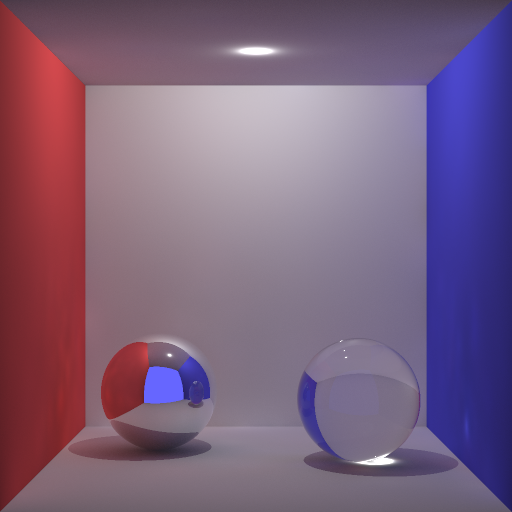
\includegraphics[width=\textwidth]{./images/renders/cornell_box.png}
	\caption{Cornell Box}
	\end{subfigure}

	\begin{subfigure}[b]{0.6\textwidth}
	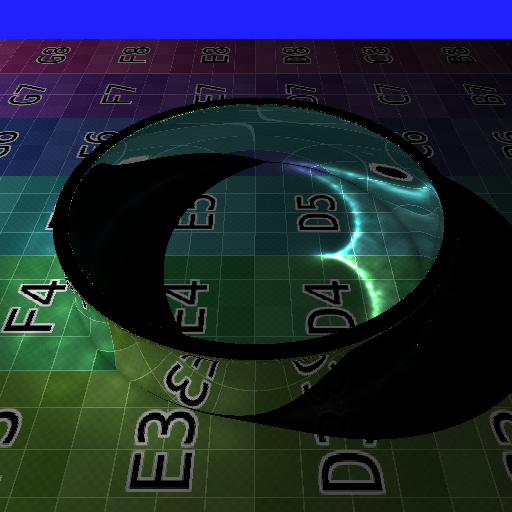
\includegraphics[width=\textwidth]{./images/renders/caustic_ring.png}
	\caption{Caustic Ring}
	\end{subfigure}
\end{figure}

\begin{figure}
\centering
	\begin{subfigure}[b]{0.6\textwidth}
	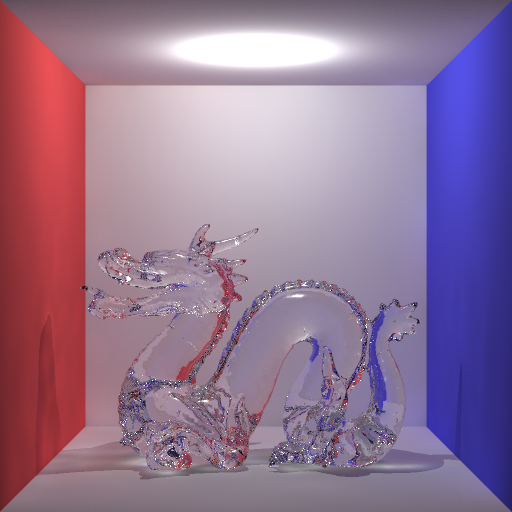
\includegraphics[width=\textwidth]{./images/renders/dragon.png}
	\caption{Stanford Dragon}
	\end{subfigure}

	\begin{subfigure}[b]{0.6\textwidth}
	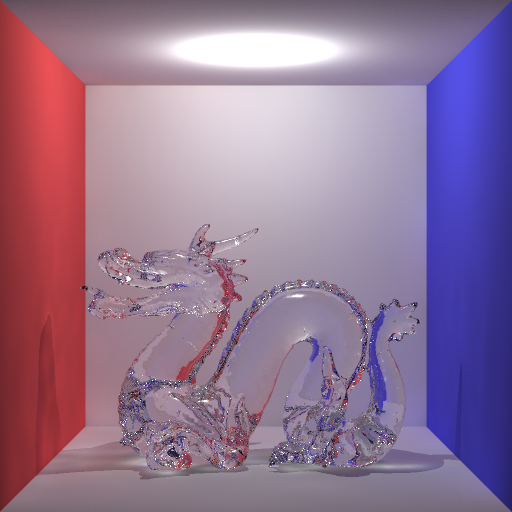
\includegraphics[width=\textwidth]{./images/renders/dragon.png}
	\caption{Stanford Dragon}
	\end{subfigure}
\end{figure}

\missingfigure{participating media low}
\missingfigure{participating media high}
